% HEADER
\documentclass[class=article, crop=false]{standalone}
\usepackage{00_Preamble/frr_preamble}

% Packages
\usepackage{titlesec}
\usepackage{hyperref}
\usepackage{float}
\usepackage{graphics}
\usepackage{placeins}
\usepackage{adjustbox}
% END HEADER

\begin{document}
	\subsection{System Testing and Verification}
	\label{subsec:system_testing_and_verification}
	
	
	
	\subsubsection{Frame and Drive Testing}
	
	\begin{wrapfigure}{r}{0.35\textwidth}
		\centering
	 	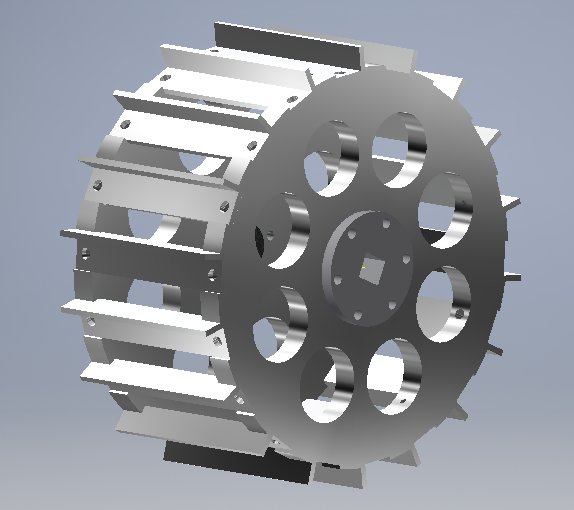
\includegraphics[width=0.30\textwidth]{09_Figures/final_wheel.png}
	 	\caption{CAD Model of Final Wheel Assembly}
	 	\label{fig:final_wheel}
	\end{wrapfigure}	
	
	The wheels must be tested for their performance in traversing the Martian terrain. It must be verified that there is not a lot of wheel slippage and that the autonomy sensors can accurately measure angular rotation. This, along with the optimal turning radius and the robot's ability to escape steep ditches, will be tested by driving the robot in a sandy environment. The environment will have obstacles similar in size to the ones on the RMC field, with sand and gravel representing the BP-1 and icy regolith, respectively.

The wheels were designed to be strong enough to carry the maximum allowed robot weight of 80 kg.  As a result, the wheels may be unnecessarily strong. The wheels' structural integrity will be tested in extreme conditions, where 50+ kg of gravel will be stored on the robot, so that the weight and power consumption can be reduced in future designs if possible.

	\subsubsection{Depositing System Testing}
	
	The depositing system must be tested to verify that it can store icy regolith, filter excess BP-1, and deposit icy regolith in the collection bin. This will be done by carrying out competition trial runs in a sandy environment. It will also be tested that the nylon mesh correctly filters BP-1 while retaining the icy regolith. A primary concern is that the filtered BP-1 will interfere with electrical components, as an electrical box containing most of the power distribution system rests directly under the conveyor. It will be verified that the electrical box was made dustproof by pouring dust onto the conveyor while the robot is running and confirming that all power systems remain active.
	Due to size constraints near the front of the frame, the conveyor had to be driven by a long roller chain at the back (Figure \ref{fig:conveyor_chain}). The chain may not have enough tension and the drive shaft could skip, which would cause the two roller chains that drive the conveyor to misalign. It must also be confirmed that icy regolith can be carried up the conveyor without sliding back down the incline. The nylon mesh will have a low coefficient of friction with the icy regolith, and small supports may need to be added to lift the icy regolith to the height of the collection bin. These factors will be tested by driving the conveyor under heavy icy regolith loads in competition trial runs.
	
	\FloatBarrier
		\begin{figure}[h]
			\centering
			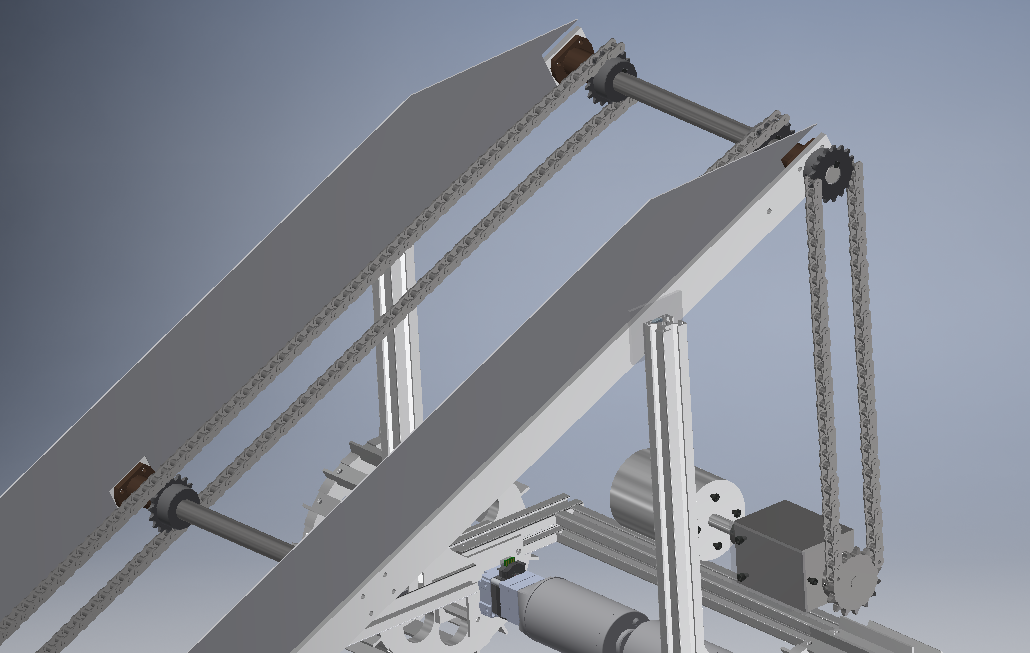
\includegraphics[width=0.5\linewidth]{09_Figures/conveyor_roller_chain.png}
			\caption{Conveyor Chain with Potential Tension Problems}
			\label{fig:conveyor_chain}
		\end{figure}
		\FloatBarrier
		
				
		\subsubsection{Excavation Testing}
		
		It is essential that the excavation system performs well, as the rest of the systems are dependent on successful icy regolith excavation. The greatest concern raised during preliminary auger testing was that icy regolith would get stuck between the PVC pipe and auger and jam the system. If this were to happen during the competition, the auger would have to be reversed to unload the icy regolith. This would cost time and potentially damage the excavation system. Before competition, it will be verified that the PVC pipe performs well at funneling icy regolith without jamming. 
		
		\subsubsection{Robot Controller Testing}
		
		The robot controller testing will ensure that the controller can receive data from all sensors and control the output of all actuators. As each sensor and actuator is mounted on the frame of the robot, the IO functionality will be tested with the robot controller. Each actuator will be moved through its full range of motion to ensure that the control inputs are functioning correctly.
		
		\subsubsection{Autonomy Testing}
		
		In order to verify the autonomy system, each layer of the autonomy stack must be tested separately. The first tests involve collecting data from each sensor to quantify the noise of each sensor. Each sensor is set in a controlled testing environment with known parameters. The error between the true measurement and the sensor measurement is logged over time and a histogram is generated from the data.
		
	The camera with the AruCo marker was tested according to the protocol. The camera was held 2.32 meters away from the marker and tracking was tested with gaussian blur and bilateral filtering. The maximum tracking range and angle were measured for each filtering technique. In an environment with minimal dust, the two filtering techniques performed equally as well as the data without filtering. However, the bilateral filtering technique performs better in a dusty environment at the cost of computational power.
	
	Once the sensors are mounted on the robot, the sensors will also be tested in a dynamic environment to determine the effect of vibration on the accuracy of the sensor data. The error distributions from the sensor data will be used to generate sensor models for the EKF SLAM algorithm.
	
	The next layer to test is the SLAM layer. Once the sensor models are built, the SLAM algorithm will be verified by running the robot in an environment similar to the competition arena. The robot will be controlled by a human driver and the accuracy of the localization will be tested by driving the robot in a loop, a task similar to one the robot will perform autonomously during the competition. If the robot pose and map diverge, the parameters for the sensor models will be tweaked until the model is stable.
	
	The path planning algorithm has been tested through simulation. Multiple virtual environments have been created for the robot to traverse. These were used to eliminate bugs in the algorithm code and to determine the effect of parameters on the performance of algorithm. Once the SLAM algorithms are validated on the robot, the system specific parameters for path planning will be determined by running the robot through a preconfigured environment with obstacles.


		
	
			
	
	

\end{document}
